In addition to knowing how the ``internal'' parameters of the problem (resolution and problem size) affect solution time, it is also important to understand how aspects of the environment can affect solution times. For this reason, various aspects of the obstacle representation and their relationship to the trajectory location are investigated in terms of the effect on solve time.

The obstacle avoidance constraint is formulated as a Mixed-Integer Linear constraint by constraining every point of the trajectory to be within one of several obstacle free polyhedral regions. An obvious avenue of investigation is to explore the effect of the number of polyhedral regions on the solve time. Another less obvious avenue is the effect of the relative position of an obstacle (encapsulated by the relative position of the obstacle free regions) to the trajectory, and specifically to the beginning and end points of the trajectory as the solution is constrained to be at both points.

\subsection{Number of Regions} \label{ssec:number_of_regions}
While the effects of problem size were more extensively studied without the presence of obstacles, the presence of the obstacle avoidance constraints can affect the solve time, and so it is useful to have a few points of reference with regards to problem size for a more in depth study. The results of this investigation are shown in Fig. \ref{fig:number_of_regions}.
\begin{figure}
    \centering
    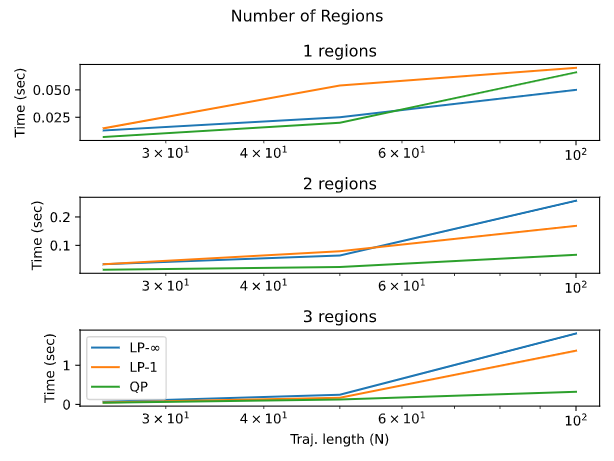
\includegraphics[width=\linewidth]{figs/Number_of_Regions.png}
    \caption{The effects on the number of regions for a selection of problem sizes. The resolution is scaled by the problem size in order to maintain a 10 second trajectory, with the step size being 0.1 seconds for the problem with 100 steps. Note that the solve time of the QP with three regions and 50 steps is about 125 ms.}
    \label{fig:number_of_regions}
\end{figure}

Of primary note is that the QP formulation performs the best in these cases with these problem sizes. Based on the previous results with problem size, however, it is expected that the QP will not scale as effectively to larger problem sizes. While the best solve times are with only 25 steps over the 10 second horizon, this results in a step size of 0.4 seconds. This is still reasonable, as demonstrated by the resolution comparison in Subsection \ref{ssec:obj_val}, but the increase in required solve time is not substantial when using 50 steps while the resulting step size is half the size (0.2 seconds). This indicates that a problem size of 50 steps may be a good compromise point.

\subsection{Obstacle Placement} \label{ssec:obstacle_placement}
In addition to the number of regions, the physical relationship between these regions and the trajectory also can have an effect on the solve time of the optimization. As may be expected, if the input trajectory already lies completely within the obstacle free regions the solve time is quite fast. Similarly, if there is a ``significant'' amount of space in between the constrained points of the trajectory (in this case the beginning and ending points of the trajectory) and the location of the obstacle (or where the trajectory is outside the obstacle free regions) the optimization runs relatively quickly.

However, when one (or more) constrained points of the trajectory are too near an obstacle the solve time can be greatly affected. This is shown in Fig. \ref{fig:obstacle_placement} where four cases are shown, where the obstacle is in the middle of the trajectory, in the middle of a short trajectory, near the beginning of the trajectory, and near the end of the trajectory. This results in the obstacle being ``far'' from both of the constrained points (beginning and end), ``close'' to both, ``close'' to the beginning, and ``close'' to the end, respectively. The resulting trajectories can be seen in Figs. \ref{fig:obstacle_mid} - \ref{fig:obstacle_end}.

\begin{figure}
    \centering
    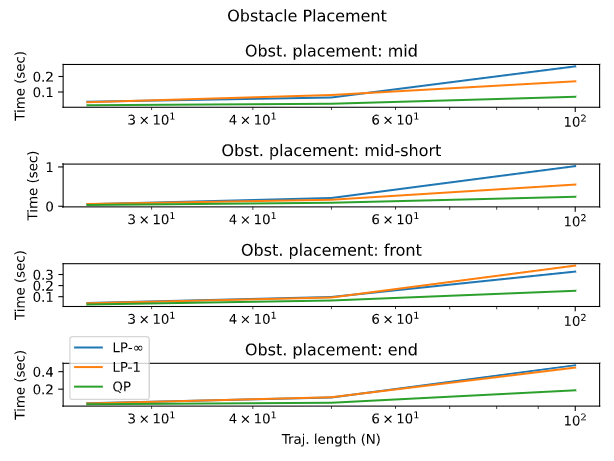
\includegraphics[width=\linewidth]{figs/Obstacle_Placement.png}
    \caption{The effect on the solve time of the placement of the obstacle in relation to the trajectory.}
    \label{fig:obstacle_placement}
\end{figure}

Again, it can be seen in the figure that the QP formulation is the fastest for solving the optimization for these situations. Also similar to the previous results, the problem size of 50 steps strikes a balance between solve time and step size, although one that is not as convincing as previously. Given the results of both investigations, it would seem that using a QP formulation with a 50 step horizon is a good choice for an MPC formulation. This choice allows for rapid online updates with a horizon that allows for quality solutions. Actual MPC validations must be performed as there may be additional factors not accounted for in these tests, but these tests provide a good starting point and intuition for investigating the MPC performance under its various hyper-parameters.

\begin{figure}
    \centering
    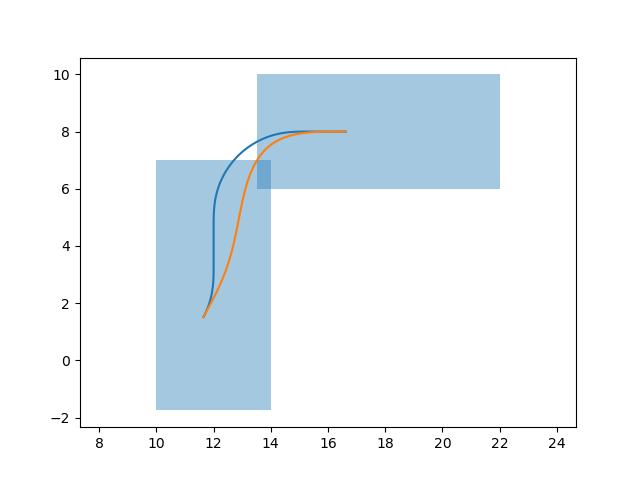
\includegraphics[width=\linewidth]{figs/mid_0_14.png}
    \caption{The obstacle is in the middle of the trajectory, i.e., far from the beginning and end points that are constrained in place.}
    \label{fig:obstacle_mid}
\end{figure}

\begin{figure}
    \centering
    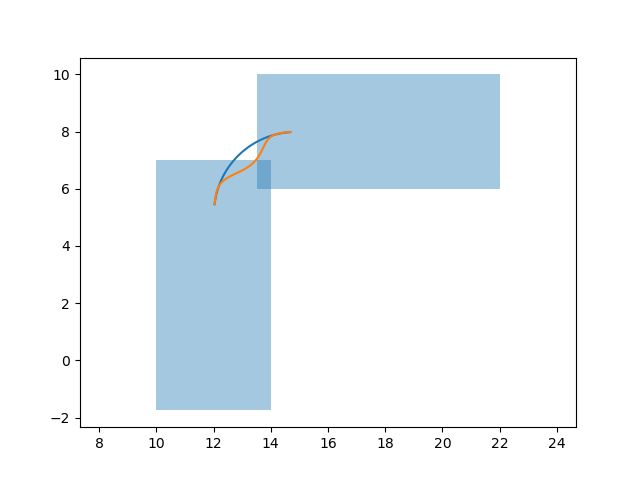
\includegraphics[width=\linewidth]{figs/mid_short_0_39.png}
    \caption{The obstacle is in the middle of a shorter trajectory, i.e., close to both the beginning and end points that are constrained in place.}
    \label{fig:obstacle_mid_short}
\end{figure}

\begin{figure}
    \centering
    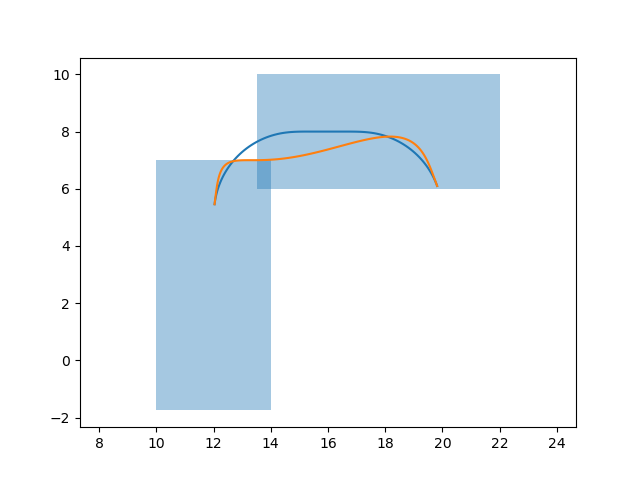
\includegraphics[width=\linewidth]{figs/beginning_0_31.png}
    \caption{The obstacle is in the beginning of the trajectory, i.e., close to the beginning point, but far from the end point.}
    \label{fig:obstacle_beginning}
\end{figure}

\begin{figure}
    \centering
    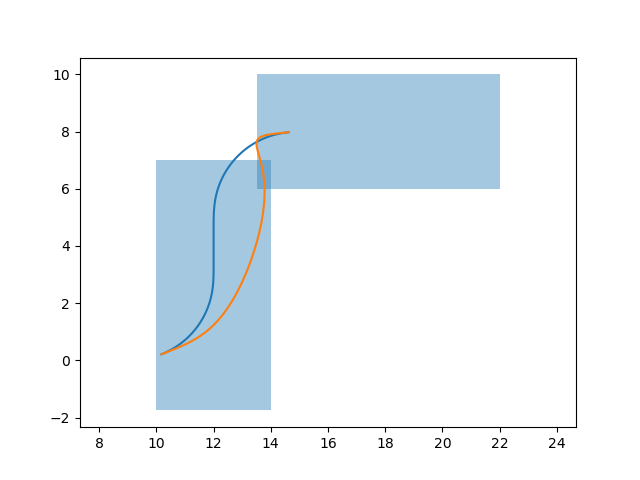
\includegraphics[width=\linewidth]{figs/end_0_26.png}
    \caption{The obstacle is in the end of the trajectory, i.e., far from the beginning point and close to the end point.}
    \label{fig:obstacle_end}
\end{figure}
